\section{Introduction}

In our Praktikum, we use a robot simulator which is embedded in the Neurorobotics Platform (NRP). The NRP is a web platform and it uses the Gazebo robotics simulator. Gazebo offers the ability to simulate robots in complex environments and uses a non-deterministic physics engine to simulate gravity, inertia, etc.
ROS serves as the interface for the robot.
The NRP has an interactive mode to develop experiments and a non-interactive mode (virtual coach) for optimizations.

The simulation consists of a robot arm with six joints and a five finger hand. The robot arm is attached to the back of a table. Seen from the robot arm, there is a cylinder on the front right corner of the table. 
The aim of our Praktikum is to let the robot arm learn how to throw the cylinder as far away from the table as possible.
The robot arm and the cylinder are shown in figure \ref{fig:challenge}.

\begin{figure}
	\begin{center}
		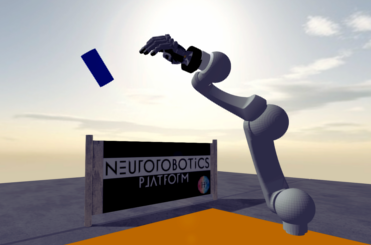
\includegraphics[width=0.4\textwidth]{hbpprak_2018}
	\end{center}
	\caption{The robot arm throwing the cylinder away from the table.}
	\label{fig:challenge}
\end{figure}

This submission report is structured as follows: section \ref{sec:motivation} motivates our choice of algorithms for solving the  Praktikum challenge. Sections \ref{sec:EA} and \ref{sec:MCMC} describe these algorithms in general. Sections \ref{sec:PrepareHit}, \ref{sec:Throw}, and \ref{sec:Windup} describe our approaches for solving the challenge.
Section \ref{sec:problems} discusses problems which occured during implementation and execution of these approaches. Finally, section \ref{sec:conclusion} summarizes the approaches and draws a conclusion.
